\documentclass[border=10pt]{standalone}

\usepackage{tikz}
\usepackage{tikzsymbols}
\usetikzlibrary{calc,patterns,shapes.geometric}

\def\centerarc[#1](#2)(#3:#4:#5){\draw[#1] ($(#2)+({#5*cos(#3)},{#5*sin(#3)})$) arc (#3:#4:#5);}

\begin{document}
	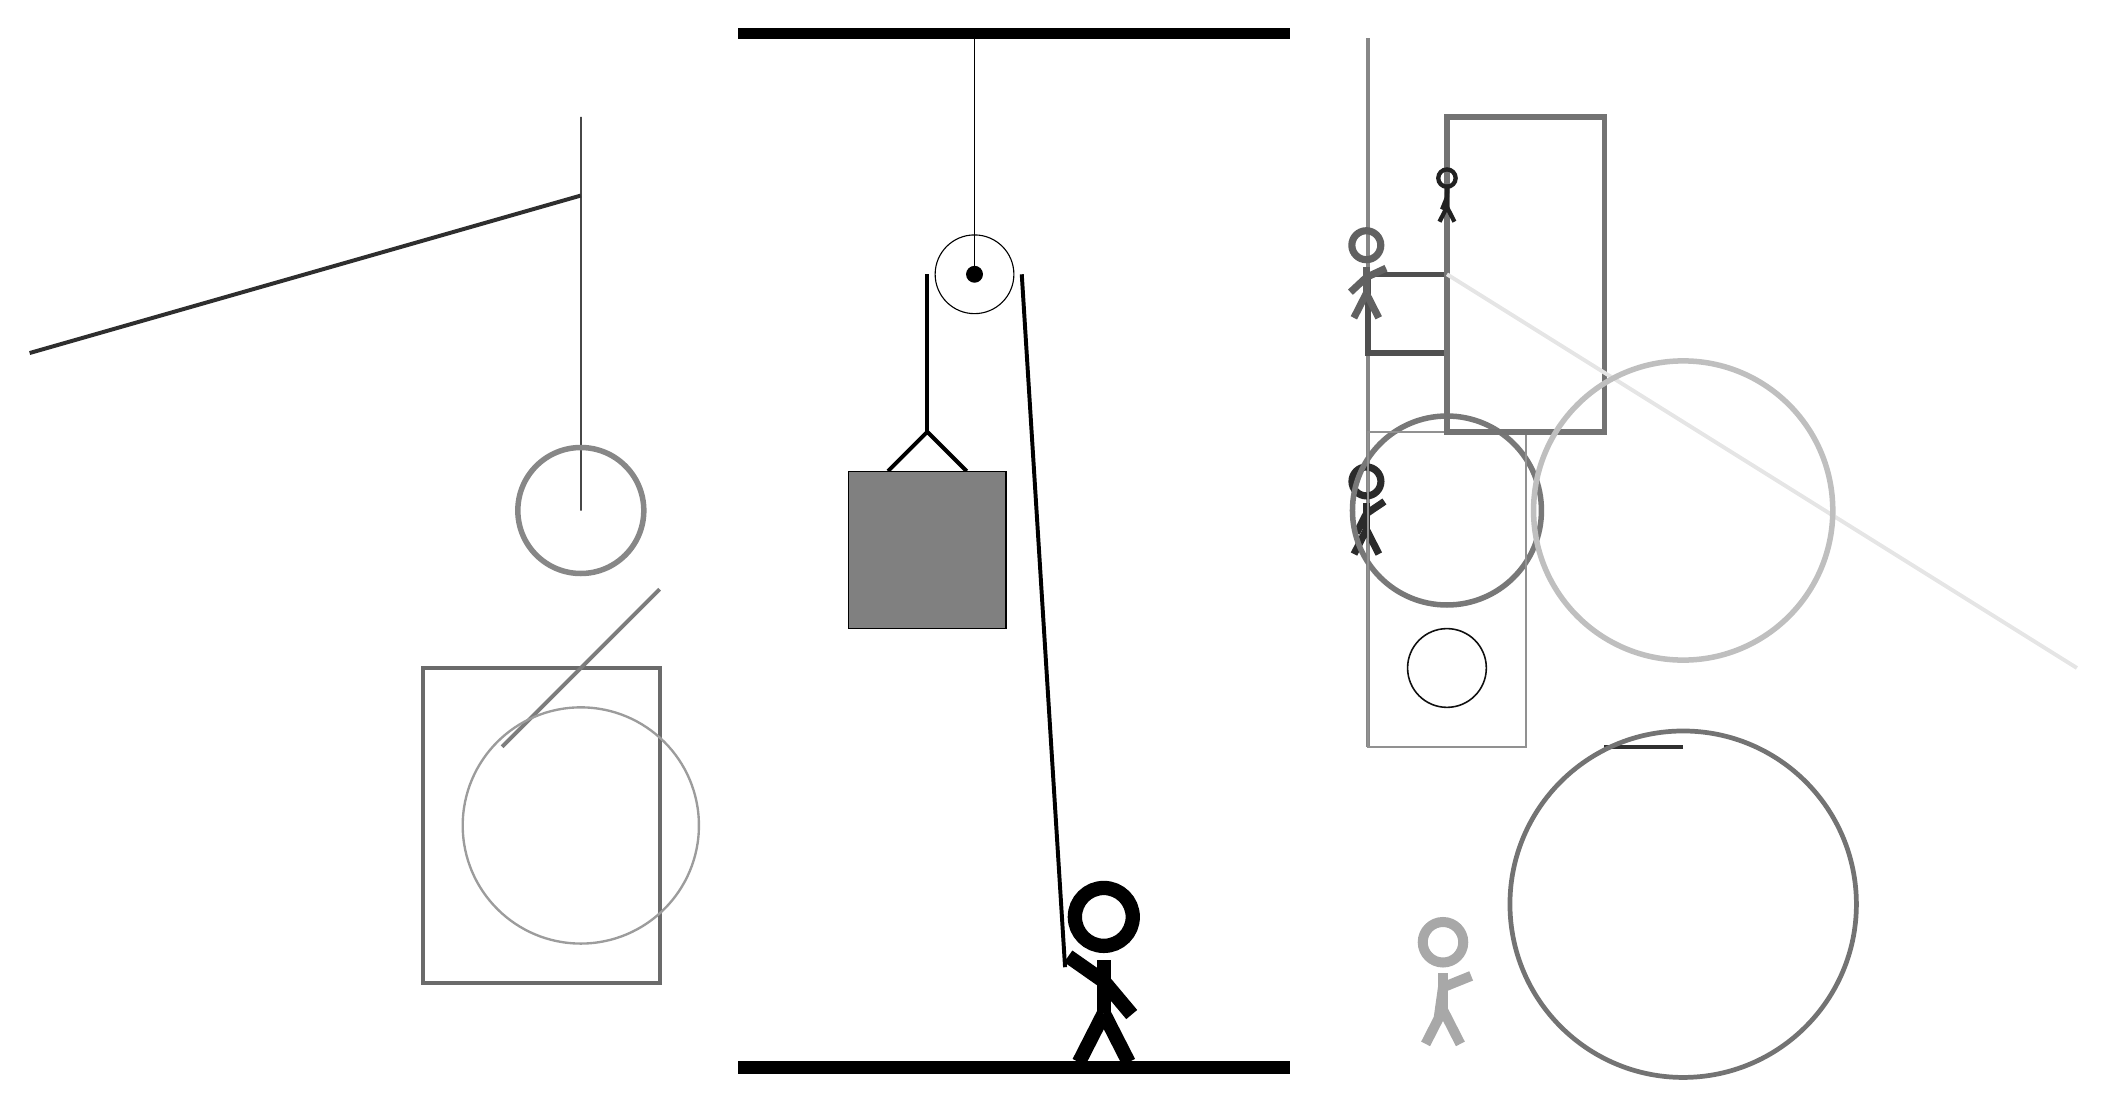
\begin{tikzpicture}
		%%%%% START %%%%%
		
		\draw[fill=black] (-2, 10) rectangle (5, 10.125);
		
		\draw[line width=0.5mm, color=black!47](6, 10) -- (6, 1);
		
		\node[line width=0.5mm, color=black!83] at (6, 4) {\Strichmaxerl[5][63][34]};
		\draw [line width=0.7mm, color=black!53](7, 4) circle (1.2);
		\draw[line width=0.7mm, color=black!69] (7, 7) rectangle (6, 6);
		\draw[line width=0.5mm, color=black!58] (-3, -2) rectangle (-6, 2);
		\node[line width=0.3mm, color=black!34] at (7, -2) {\Strichmaxerl[7][82][22]};
		\draw[line width=0.3mm, color=black!43] (6, 1) rectangle (8, 5);
		\draw[line width=0.7mm, color=black!55] (7, 5) rectangle (9, 9);
		\draw[line width=0.5mm, color=black!10](7, 7) -- (15, 2);
		\draw[line width=0.5mm, color=black!81](10, 1) -- (9, 1);
		\draw[line width=0.2mm, color=black!72] (-4, 9) rectangle (-4, 4);
		\draw [line width=0.7mm, color=black!25](10, 4) circle (1.9);
		\draw [line width=0.6mm, color=black!55](10, -1) circle (2.2);
		\draw[line width=0.5mm, color=black!82](-4, 8) -- (-11, 6);
		\draw [line width=0.7mm, color=black!47](-4, 4) circle (0.8);
		\draw[line width=0.5mm, color=black!51](-5, 1) -- (-3, 3);
		
		\node[line width=0.6mm, color=black!62] at (6, 7) {\Strichmaxerl[5][43][25]};
		\draw [line width=0.2mm, color=black!94](7, 2) circle (0.5);
		\node[line width=0.5mm, color=black!87] at (7, 8) {\Strichmaxerl[3][68][88]};
		\draw [line width=0.3mm, color=black!39](-4, 0) circle (1.5);
		
		\draw (1, 7) circle (0.5);
		\draw[fill=black] (1, 7) circle (0.1);
		\draw (1, 10) -- (1, 7);
		
		\draw[line width=0.5mm] (-0.1, 4.5) -- (0.4, 5.0) -- (0.9, 4.5);
		\draw[fill=black!50] (-0.6, 4.5) rectangle (1.4, 2.5);
		
		\draw[line width=0.5mm] (0.4, 7) -- (0.4, 5.0);
		\centerarc[line width=0.5mm](1, 7)(0:180:0.6);
		\draw[line width=0.5mm](1.6, 7) -- (2.15, -1.8);
		
		\node at (2.6, -1.9) {\Strichmaxerl[10][-35][-50]};
		
		\draw[fill=black] (-2, -3) rectangle (5, -3.15);
		
		%%%%% END %%%%%
	\end{tikzpicture}
\end{document}